\section{Opgave 3}
\subsection{Beskrivelse og Design}
	
	Man kan simulerer den nummeriske værdi af $\pi$ ved at ``kaste'' en nål på et gulv med linjer (ex. revner mellem brædderne).
	Linjerne skal være parallelle og have en afstand, der er det dobbelte af nålens længde.
	Man tæller så, hvor mange gange nålen lander, så den ligger hen over en linje. forholdet mellem antalet af kast $t$
	og antallet af gange, nålen krydser en linje $n$ giver så $\pi \approx \frac{t}{n}$.
	
	Se evt \url{http://en.wikipedia.org/wiki/Buffon's_needle}.
	
	Vi laver et program, der simulerer disse kast.
	For hvert kast bør genereres en tilfældig position for nålen og en tilfældig vinkel for denne,
	dette kan dog simplificeres lidt, vi behøer for det første kun kigge på en enkelt dimmension.
	Desuden er det kun interessant at kigge på kast, hvor nålen er linjeafstanden væk fra en bestemt linje.
	Nålen fylder desuden det samme i retningen vinkelret på linjerne skråt den ene vej, eller skråt den anden,
	det er derfor kun nødvendigt at genererer vinkler i $[0;\frac{Pi}{2}]$
	
	For hvert kast udføres således følgende funktion:
	
	\begin{lstlisting}[caption=Pseudokode for hvert kast]
Sæt nålens længde til 1
Sæt linjeafstanden til 2
Sæt nålens centrum til et tilfældigt tal mellem 0 og linjeafstanden
Sæt nålens vinkel til et tal mellem 0 og PI/2

Hvis nålen rører linjen i enten den ene eller den anden ende
	læg en til antallet af ramte forsøg
	\end{lstlisting}

	Nålen rammer kun stregen i følgende to situationer, illustreret på figur~\ref{fig:3a01}:
	
	Nålen stikker ``tilbage'' og rammer en linje ``bag'' den, dvs
	\begin{equation}
	needleCenter \leq \cos(needleAngle)\cdot \frac{needleLength}{2}
	\end{equation}
	
	Eller nålen stikker ``frem'' og rammer en linje ``foran'' den, dvs
	\begin{equation}
	lineSpacing - needleCenter \leq \cos(needleAngle)\cdot \frac{needleLength}{2}
	\end{equation}

	\begin{figure}[h!]
	  \centering
	      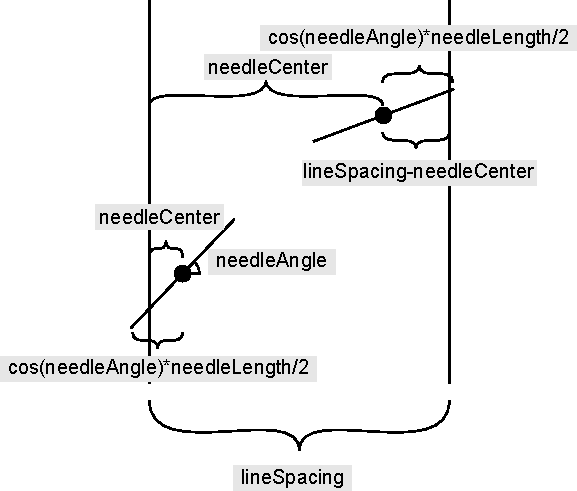
\includegraphics[width=0.5\textwidth]{3a01}
	  \caption{Illustration af kast med \emph{Buffons Nål}}\label{fig:3a01}
	\end{figure}


\subsection{Programtest}
	For at teste programmet's korrekthed skal følgene egenskaber verificeres:
	\begin{enumerate}
		\item Programmet afbrydes når kommandoen "exit" modtages
		\item Programmet ignorerer alle inputs, der ikke er positive tal (mindre end $2^31-1$)
		\item Programmet skal estimnerer $\pi$
	\end{enumerate}
	Der findes endnu et tilfælde, der dog ikke vil blive testet, dette er at programmet modtager en tekstreng der er for stor til at kunne håndteres.
	Dette er dog meget usandsynligt eftersom Java kan håndtere meget store tekstrenge og programmet ville tage meget lang tid om at evaluere den største tekstreng der kan være i input-bufferen. \\
	
	For testpunkt nr. 1 indtastes "exit" kommandoen imens programmet venter på input og imens programmet er igang med at simulere en lang række kast.
	Dette giver følgene outputs:
	\begin{lstlisting}[caption=Output fra testsekvens]
Type 'exit' to exit
Enter a positive number of iterations: exit
Done!
	\end{lstlisting}
	Og imens programmet arbejder på mange kast:
	\begin{lstlisting}[caption=Output fra testsekvens imens programmet evaluerer]
Type 'exit' to exit
Enter a positive number of iterations: 10000000
exit
Result: 
 	iterations = 10000000
	Hits = 3183207
	Ratio = 3.141485929127449
	Distance to Math.PI: 1.0672446234405442E-4
Enter a positive number of iterations: Done!
	\end{lstlisting}
	Det ses at programmet regner færdigt før det afsluttets, hvilket også fremgår af kildekoden.\\
	
	Testpunkt 2. Vi tester om inputs, der ikke er positive tal forkastes:
	\begin{lstlisting}[caption==Output fra testsekvens 2]
Type 'exit' to exit
Enter a positive number of iterations: -1
Enter a positive number of iterations: 0
Enter a positive number of iterations: Help Im Trapped In A Universe Factory!
Enter a positive number of iterations: exit
Done!
	\end{lstlisting}
	
	Testpunkt 3. Da vi ikke går dybere ind i matematikken bag \emph{Buffons nål} er den bedste test herpå at kaste nok gange:
	\begin{lstlisting}[caption==Output fra testsekvens 2]
Type 'exit' to exit
Enter a positive number of iterations: 100000000
Result: 
 	iterations = 100000000
	Hits = 31831422
	Ratio = 3.141549881120611
	Distance to Math.PI: 4.27724691820508E-5
Enter a positive number of iterations: 100000000
Result: 
 	iterations = 100000000
	Hits = 31827564
	Ratio = 3.1419306862441623
	Distance to Math.PI: 3.380326543691581E-4
Enter a positive number of iterations: 100000000
Result: 
 	iterations = 100000000
	Hits = 31835616
	Ratio = 3.1411360157127164
	Distance to Math.PI: 4.5663787707672654E-4
Enter a positive number of iterations: exit
Done!
	\end{lstlisting}
	Det ses iøvrigt at estimeringen ikke bliver den samme hver gang, men stadig relativt tæt på $\pi$.